\section{Experimental Details}

	\subsection{Equipment}
		The experiment apparatus consisted of a sodium discharge lamp, a glass grating, a telescope, a power supply for the discharge lamp and a circular scale. 
		\\
		\\
		The sodium discharge lamp provided incident light for us to observe the spectral lines, the glass grating was used to perform transmission diffraction to separate the wavelengths of incident light, the telescope was used to look though the discrete spectra of sodium and the circular scale was used to measure the angle of the telescope with respect to the glass grating. The complete apparatus can be seen in the figure below.
		\\
		\begin{figure}[h!]
			\centering
			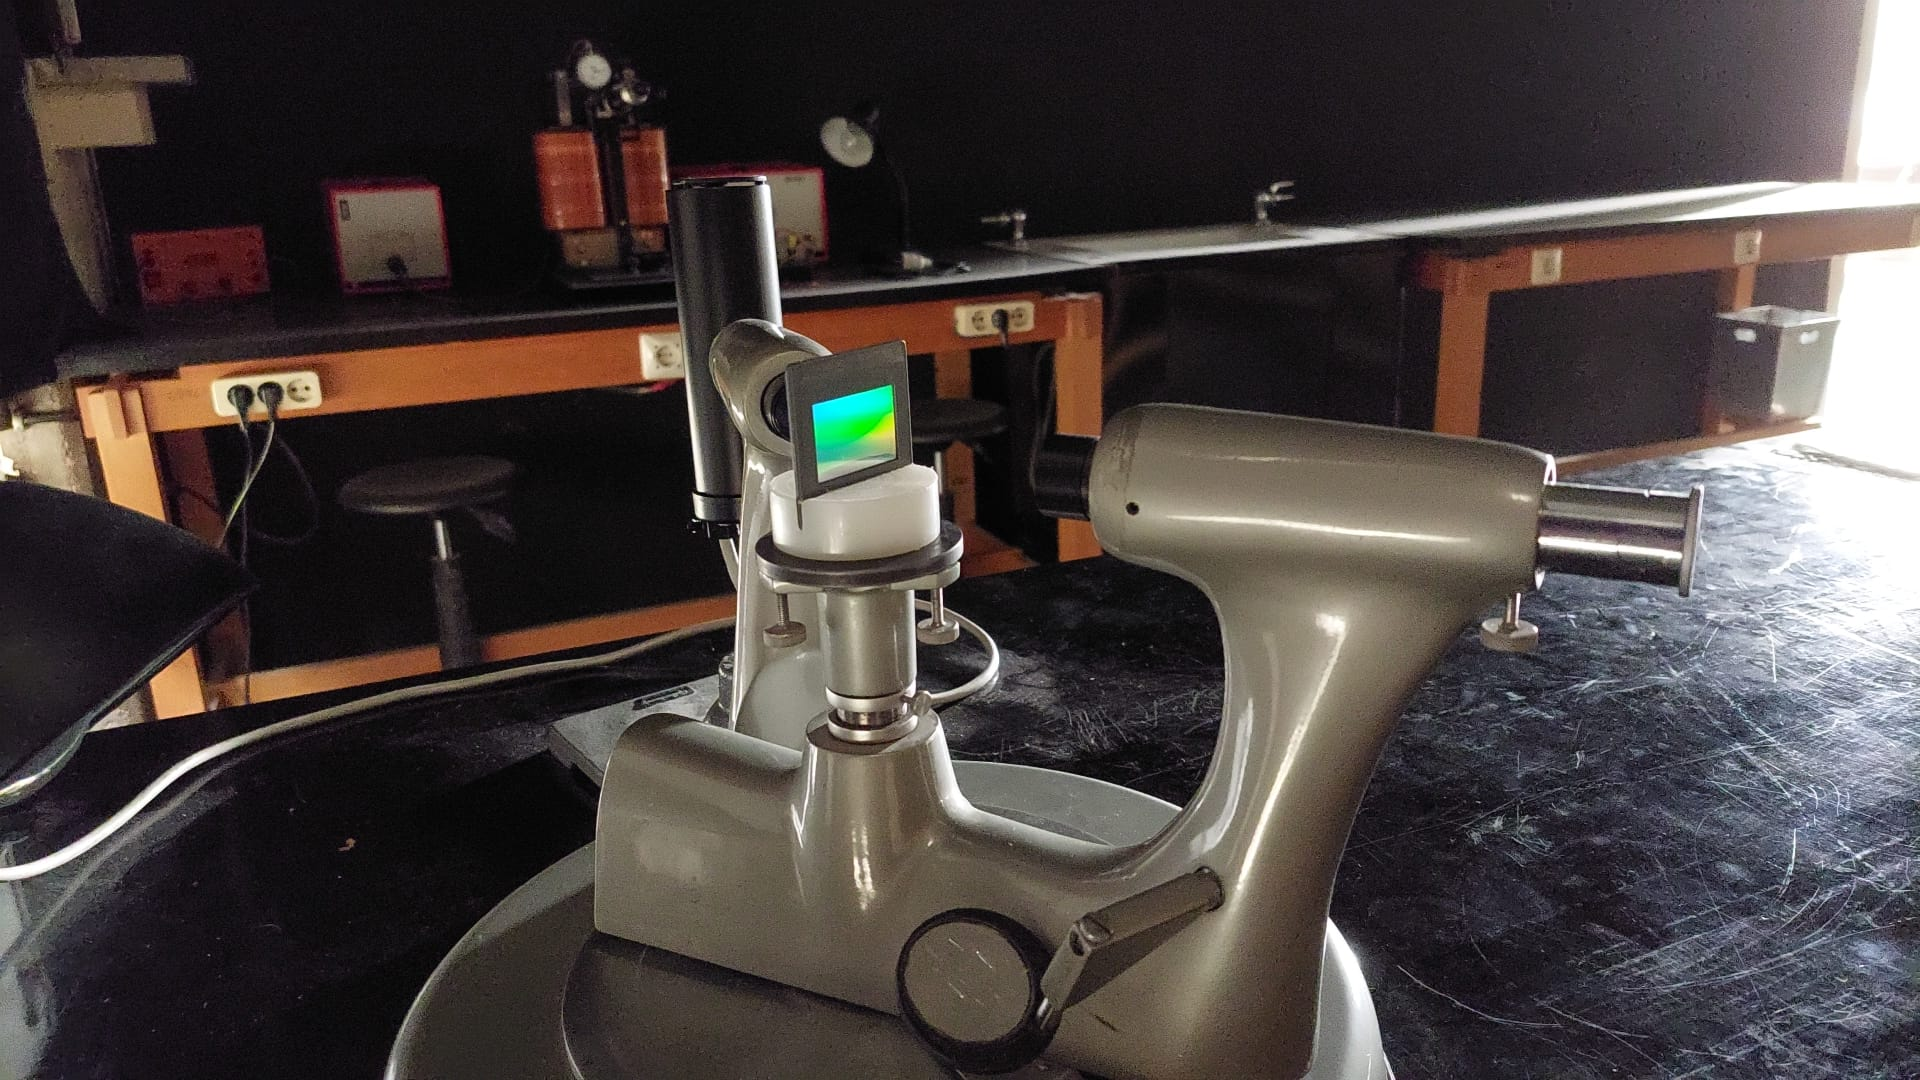
\includegraphics[width=8cm]{images/as_setup.jpeg}
			\caption{The Atomic Spectra experiment apparatus.}
			\label{fig:as_setup}
		\end{figure}
	
	\subsection{Procedure}
		The first part of the experiment consisted of adjusting the glass grating perpendicular to the line of sight and recording the angles in which we observe certain spectral lines. 
		\\
		\\
		The second part of the experiment consisted of adjusting the glass grating to a sixty degree angle and recording the angles in which fine structure splitting was present. 
